
\chapter{Methodology}
\begin{refsection}

This chapter provides the methodology for developing the prototype for the spatiotemporal localization model for an \gls{ar} navigation system in \gls{cspc}, including data collection, pre-processing, \gls{ml} model training and testing, and performance evaluation.

\section{Research Design}

Constructive research design is a strategy for creating new constructs or systems that build on existing knowledge, concepts, or methods to address specific problems or challenges. It involves developing innovative solutions by combining and adapting well\-established theories, techniques, and models to solve real-world problems. This design often relies on a combination of existing tools, knowledge, and frameworks, where researchers adapt and reassemble them into novel constructs or systems. In this process, the research seeks not only to develop theoretical understanding but also to create practical, tangible, functional solutions that can be implemented in real-world settings. This design is particularly relevant in fields where continuous innovation and development are required and where applying existing knowledge to new contexts can lead to breakthroughs in solving emerging problems \cite{crnkovic2010}.

This study will adopt a constructive research design to develop a spatiotemporal localization model for an \gls{ar} navigation system at \gls{cspc}, using \gls{cnn} and \gls{lstm} networks. The constructive research design suits the study well, as it involves combining different existing models and algorithms to create a system that addresses the problem stated in Chapter 1.2. The artifact in this study is a spatiotemporal localization model integrated into a mobile AR navigation application. It is designed to determine user location based on visual cues and sensor data (e.g. rotation vector) collected from the mobile device, without the need for internet connectivity or \gls{gps}. This approach ensures that the \gls{ar} navigation system operates independently of real-time data transmission, making it robust in environments with limited or no network connectivity.

Adopting a constructive research design allows researchers to build on existing methodologies while innovating and developing a new solution that addresses the specific challenges of \gls{ar} navigation in an educational setting. This approach facilitates the creation of an artifact that can function independently of conventional data sources, ensuring that the \gls{ar} navigation system is reliable and effective in dynamic and offline environments. Drawing on existing knowledge and adapting it creatively, the study aims to provide a significant contribution to the field of \gls{ar} navigation and spatiotemporal localization.

\section{Theorems, Algorithms, and Mathematical Models}

In computer science, theorems, algorithms, and mathematical models lay the foundation for \gls{ml} models. This study will use \gls{cnn} together with \gls{lstm} networks for spatiotemporal localization, highlighting their utility in feature extraction and sequential learning for spatiotemporal awareness. In particular, this study will use ResNet-50, which is based on \gls{cnn}, and a regular \gls{lstm} model.

\subsection{ResNet-50 Architecture}

Residual Networks, or ResNets, were introduced to overcome the challenges of training very deep neural networks, particularly the degradation problem, where adding more layers to a network leads to worse performance rather than improved accuracy. Proposed by \citeauthor{he2015deepresiduallearningimage} \citeyear{he2015deepresiduallearningimage}, ResNet introduces the concept of residual learning, where the layers are designed to learn the residual or the difference between the input and the desired output rather than learning the output directly. This is achieved through the use of shortcut connections that skip one or more layers, enabling the network to pass information directly from the earlier to the later layers. These identity shortcuts help preserve gradients during training, effectively mitigating the vanishing gradient problem and making it possible to train networks with hundreds or even thousands of layers \cite{he2015deepresiduallearningimage}.

\begin{figure}[H]
    \centering
	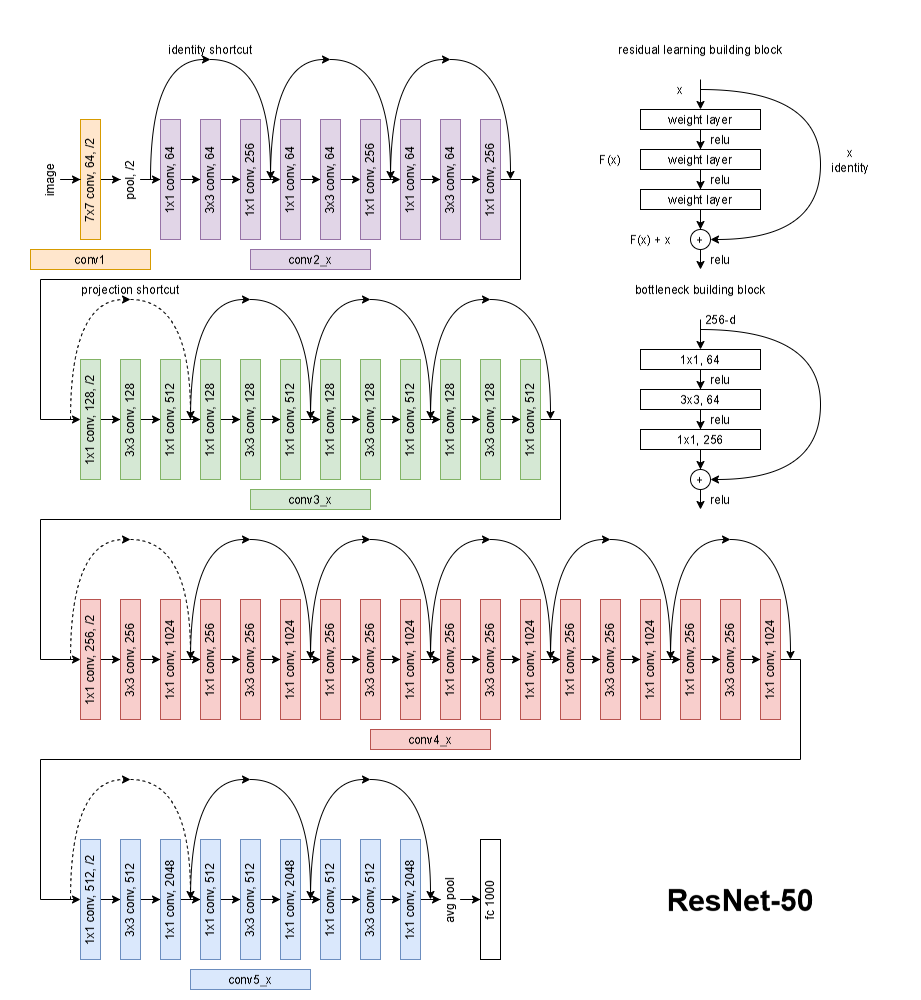
\includegraphics[width=0.85\textwidth]{figures/resnet.png} 
	\caption[ResNet-50 Architecture]{Detailed diagram of the ResNet-50 Architecture.}
	\label{fig:firstFig}
\end{figure}

\ref{fig:firstFig} shows the architecture of ResNet-50, a variant of the Residual Networks architecture consisting of 50 layers, specifically utilizing a bottleneck design that includes three layers per residual block (1x1, 3x3, and 1x1 convolutions). This setup allows for dimension reduction for lighter computation in the later layer and then dimension expansion for the preservation of the block input size. This distinguishes it from shallower versions of ResNet such as ResNet-18 and ResNet-34, which, on the other hand, use two-layer blocks and fewer overall layers, making them less computationally intensive, but also potentially less powerful. In contrast, deeper models such as ResNet-101 and ResNet-152 extend the number of layers and blocks, increasing the capacity at the cost of higher computational complexity. ResNet-50 offers a balance between depth, performance, and computational efficiency, which led the researchers to choose this particular architecture variant. It consist of five residual blocks, namely; conv1, conv2\_x, conv3\_x, conv4\_x, and conv5\_x. Each of these residual blocks output different sizes, which are 112x112, 56x56, 28x28, 14x14, and 7x7 respectively. The final fully-connected later outputs the final 1x1 output size \cite{he2015deepresiduallearningimage}.

For this study, however, the researchers decided to remove the final fully-connected classification layer, as the CNN will be used as a feature extractor instead of its usual use case in classification problems.

\subsection{Main Features of ResNet-50}

\subsubsection{Residual Learning}

ResNet-50 uses residual learning to address the degradation problem in deep networks. Instead of learning the output directly, it learns the residual (the difference between input and output) using shortcut connections. This approach improves the flow of the gradient, allowing training of deeper and more accurate networks.

In the study of \citeauthor{he2015deepresiduallearningimage} \citeyear{he2015deepresiduallearningimage}, the following formulation define the building block of ResNet as:

\begin{equation}
y = F(x, \{W_i\}) + x
\label{eq:bbresnet}
\end{equation}

Where x and y are the respective input and output vectors of the layers considered. The function \(F(x, \{W_i\})\) represents the residual mapping to be learned \cite{he2015deepresiduallearningimage}.

\subsubsection{Identity and Projection Shortcuts}

ResNet-50 uses two types of shortcut connections: identity shortcuts, which directly add input to output when the dimensions match, and projection shortcuts, which use 1×1 convolutions to adjust the dimensions when needed. These shortcuts ensure smooth information flow and support deeper architectures \cite{he2015deepresiduallearningimage}.

\subsubsection{Bottleneck Architecture}

ResNet-50 employs a bottleneck architecture, which consists of three layers: a 1×1 convolution for dimensionality reduction, a 3×3 convolution for feature extraction, and a 1×1 convolution to restore the dimensions. This design reduces computational complexity while maintaining network depth and performance \cite{he2015deepresiduallearningimage}.

\subsection{\gls{lstm} Networks}

Based on the study of \citeauthor{10.1162/neco.1997.9.1.1} \citeyear{10.1162/neco.1997.9.1.1}, \gls{lstm} is a special kind of \gls{rnn} that helps to learn patterns in long sequences of data. Regular \gls{rnn}s have trouble remembering information because they can face issues called vanishing and exploding gradients. \gls{lstm} fixes this by using a special memory cell that can choose what to keep and what to forget.

\ref{fig:secondFig} shows an \gls{lstm} cell’s three main parts, called gates: the forget gate, the input gate, and the output gate. These gates control what information to keep or ignore, allowing the network to focus on what is important. This makes \gls{lstm} suitable for tasks such as understanding languages, predicting time series, and analyzing videos \cite{10.1162/neco.1997.9.1.1}.

\begin{figure}[H]
    \centering
	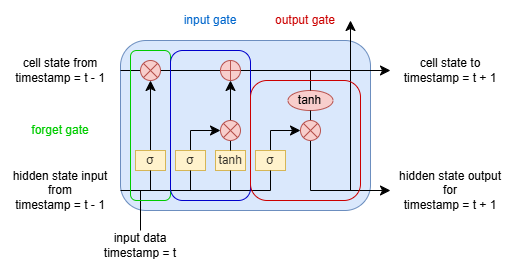
\includegraphics[width=0.85\textwidth]{figures/lstm.png} 
	\caption[An \gls{lstm} Cell]{An \gls{lstm} cell used in \gls{lstm} networks.}
	\label{fig:secondFig}
\end{figure}

\subsection{Core Components of \gls{lstm} Networks}

The core components of \gls{lstm} networks are key to their ability to process sequential data. The cell, or memory, is the central part that stores information over time. The input gate controls what new information gets added to this memory, while the forget gate decides what information should be discarded. Finally, the output gate determines which data will be sent to the next step in the process. Together, these parts help \gls{lstm}s remember important details and learn from sequences, making them great for tasks such as language understanding and time series prediction \cite{10.1162/neco.1997.9.1.1}.

In addition, the following mathematical equations define the gates of \gls{lstm} cells:

\begin{equation}
i_t = \sigma(w_i[h_{t-1}, x_t] + b_i)
\label{eq:igatelstm}
\end{equation}

\begin{equation}
f_t = \sigma(w_f[h_{t-1}, x_t] + b_f)
\label{eq:fgatelstm}
\end{equation}

\begin{equation}
o_t = \sigma(w_o[h_{t-1}, x_t] + b_o)
\label{eq:ogatelstm}
\end{equation}

Where \(i_t\) represents the input gate, \(f_t\) represents the forget gate, \(o_t\) represents the output gate, \(\sigma\) represents the sigmoid function, \(w_x\) is the weight for the respective gate(x) neurons, \(h_{t-1}\) is the output of the previous \gls{lstm} block, \(x_t\) is the input at current timestamp, and \(b_x\) are biases for the respective gates(x).

\section{Material and Evaluation Methods}

The study will use the following materials, tools, and evaluation methods in developing the spatiotemporal localization model.

\subsection{Instruments}

This section contains the dataset, hardware, and software requirements for developing the prototype for the spatiotemporal localization model.

\subsubsection{Dataset}

The study will use a dataset consisting of hyperlapse photographs of the campus and data on sensors and location. These images will be captured at a fixed interval and are sequential, so that the \gls{lstm} networks will have a sensible sequential learning from the data. Along with the images, rotation vector sensor data will be logged whenever an image is captured along with spatial coordinates.

\subsubsection{Hardware}

To support the development and testing of the proposed spatiotemporal localization model for an \gls{ar} navigation system using \gls{cnn} and \gls{lstm}, the researchers will use hardware components that meet or exceed the specifications outlined in Table 1. These components are selected to ensure efficient training of deep learning models and seamless performance of \gls{ar} features in a real-world setting.

\begin{table}[H]
\centering
\caption{Hardware Requirements}
\begin{tabular}{ll}
\hline
\textbf{Component}   & \textbf{Specification}                                                                                      \\ \hline
Processor (CPU)      & Intel i5 (or higher), 2.5 GHz or higher                                                                     \\
Memory (RAM)         & 8 GB (minimum), 16 GB recommended                                                                           \\
Storage              & 500 GB SSD or higher                                                                                        \\
Graphics Card (GPU)  & \begin{tabular}[c]{@{}l@{}}NVIDIA GTX 1060 or higher\\ (for deep learning)\end{tabular}                     \\
Sensors              & \begin{tabular}[c]{@{}l@{}}IMU sensor (Accelerometer,\\ Gyroscope, Magnetometer)\end{tabular}               \\
Mobile Device        & \begin{tabular}[c]{@{}l@{}}Android device with GPS,\\ Accelerometer, Gyroscope,\\ Magnetometer\end{tabular} \\
Camera               & \begin{tabular}[c]{@{}l@{}}High-quality camera\\ (from a Mobile Device)\end{tabular}                        \\
Python               & Version 3.13 or later                                                                                       \\
Jupyter Notebook     & Version 6.0 or later                                                                                        \\
NumPy / Pandas       & Latest version                                                                                              \\
Matplotlib / Seaborn & Latest version                                                                                              \\ \hline
\end{tabular}
\label{tab:firstTab}
\end{table}

To ensure optimal performance of the AR-based campus navigation system, several key hardware components are required. A processor with at least an Intel i5 and 2.5 GHz speed is essential for efficient data processing and model training tasks. Sufficient memory is also crucial; 8 GB of RAM is the minimum, though 16 GB is recommended to handle larger datasets and ensure smoother training operations. For data access and model storage, a 500 GB or larger solid-state drive (SSD) is preferred due to its faster read/write speeds compared to traditional hard drives. Deep learning tasks, especially those involving Convolutional Neural Networks (CNN) and Long Short-Term Memory (LSTM) models, benefit significantly from a dedicated GPU, such as an NVIDIA GTX 1060 or higher, which speeds up training and reduces computation time.

Sensor integration is a vital component of the AR system. An Inertial Measurement Unit (IMU) consisting of an accelerometer, gyroscope, and magnetometer is required to collect movement and orientation data. A compatible Android mobile device equipped with GPS and these sensors is necessary to run the AR interface and capture sensor inputs in real time during navigation. Lastly, a high-quality mobile device camera is used to capture environmental images during data collection. This visual data is essential for landmark detection and localization tasks within the AR system.

\subsubsection{Software}

\begin{table}[H]
\centering
\caption{Software Requirements}
\begin{tabular}{ll}
\hline
\textbf{Component}    & \textbf{Version/Details}        \\ \hline
Android Studio        & Ladybug (2024.2.2) or later     \\
Android SDK           & Latest stable version           \\
Programming Languages & Kotlin                          \\
Pytorch               & Version 2.7 or later            \\
TorchVision           & Compatible with Pytorch version \\
Room Database         & Latest stable version           \\
OpenCV                & Version 4.x or later            \\
Python                & Version 3.13 or later           \\
Jupyter Notebook      & Version 6.0 or later            \\
NumPy / Pandas        & Latest version                  \\
Matplotlib / Seaborn  & Latest version                  \\ \hline
\end{tabular}
\label{tab:secondTab}
\end{table}

\ref{tab:secondTab} shows the software that will be used to develop the underlying technology that will enable the \gls{ar} navigation system in and for \gls{cspc}; listed are the requirements and their respective categories that they fall under.

The development and deployment of the AR-based campus navigation system requires a robust set of software tools and libraries. Android Studio (Ladybug 2024.2.2 or later) serves as the primary integrated development environment (IDE) for building the Android-based AR application. It is supported by the Android SDK, which provides the sensor APIs necessary for access to GPS, accelerometer, and gyroscope. Kotlin is selected as the programming language due to its modern syntax and compatibility with Android development. For deep learning, PyTorch (v2.7 or later) is used to build and train the convolutional neural network (CNN) and long-short-term memory (LSTM) models used in spatio-temporal localization tasks. TorchVision, fully compatible with PyTorch, handles the essential image transformation processes required to train visual models.

To manage and store sensor data collected during user experiments, the Room Database is utilized. It supports structured local data storage within the Android environment. For computer vision tasks such as preprocessing or implementing features like hyperlapse, OpenCV (v4. x or later) is integrated. Python (v3.13 or later) is a core language used for backend model training, preprocessing, and evaluation processes. Additionally, Jupyter Notebook (v6.0 or later) facilitates exploratory data analysis and the visualization of results during development. Lastly, NumPy and Pandas, both at their latest versions, are indispensable for numerical operations and tabular data processing throughout the project.

\subsection{Procedure/Process}

\subsubsection{Data Collection}

The researchers will collect data using hyperlapse recordings, capturing images at regular intervals along predefined paths within the \gls{cspc} campus. Each image will be paired with timestamps, \gls{gps} coordinates, and sensor data. This dataset will be used to train the model to recognize movement patterns and landmarks over time.

\subsubsection{Data Pre-processing}

The collected data will be pre-processed by resizing images and splitting the data into training and validation sets. This will prepare the data for the \gls{cnn}-\gls{lstm} model and ensure that it is ready for training. Specifically, the images will be resized to 224x224 pixels be applied augmentation techniques such as random rotation and brightness adjustments. Sensor data on the other hand will be synchronized with image timestamps using linear interpolation.

\subsubsection{Model Training}

The proposed model is a hybrid architecture that combines \gls{cnn} (ResNet-50) and \gls{lstm} networks. The ResNet-50 component is pretrained on the ImageNet dataset and serves as a feature extractor, producing a fixed-size embedding vector for each image frame. These embeddings are then fed sequentially into a unidirectional \gls{lstm} to learn the temporal dependencies between frames.

During training, the ResNet-50 backbone is initially frozen for the first 10 epochs to allow the LSTM to learn stable temporal patterns. Afterward, the CNN is unfrozen to fine-tune both components jointly. The model is trained for 50 epochs using a batch size of 32 and the Adam optimizer with an initial learning rate of 0.001. Learning rate scheduling and early stop are applied to prevent overfitting. The training objective is to minimize the Mean Squared Error (MSE) between the predicted and actual spatial coordinates.

\subsubsection{Model Testing}

The trained model will be tested on a separate dataset to evaluate its ability to predict locations and track movement under dynamic real-world conditions. Key metrics like accuracy and localization error will be measured. Specifically, by Mean Euclidean Error, Root Mean Squared Error, and Accuracy within a tolerance radius.

\subsubsection{Model Fine-tuning}

The model will be fine-tuned based on testing results. Hyperparameters will be adjusted and specific layers re-trained to improve localization accuracy and robustness under various environmental conditions.

\subsection{Evaluation Methods}

This section will discuss the evaluation metrics that will be used to measure the performance of the proposed spatiotemporal localization model for an \gls{ar} navigation system. These include the mean Euclidean error, the root mean squared error, the navigation time, and the accuracy of the tolerance radius. These metrics will help determine the effectiveness of the system in recognizing landmarks and assisting users with accurate and efficient \gls{ar}-based navigation.

\subsubsection{Mean Euclidean Error (MEE)}

The Root Mean Squared Error computes the average squared difference between the predicted and actual coordinates. It penalizes larger errors more heavily, making it useful for evaluating sensitivity to outliers. It will be calculated using the following formula:

\begin{equation}
MEE = \frac{1}{n} \sum_{i=1}^{n} \sqrt{(x_i - \hat{x}_i)^2 + (y_i - \hat{y}_i)^2}
\label{eq:mee}
\end{equation}

Where \(n\) is the number of prediction made, \(x_i\) and \(\hat{x}_i\) are the actual and predicted coordinates in the \(x\) axis, while \(y_i\) and \(\hat{y}_i\) are the actual and predicted coordinates in the \(y\) axis. The squaring and rooting in the formula makes it so that computed value will equate to a Euclidean distance.

This metric will provide a human-friendly view of the model's correctness in identifying spatiotemporal landmarks \cite{gmd-15-5481-2022}.

\subsubsection{Root Mean Squared Error (RMSE)}

The Root Mean Squared Error computes the average squared difference between the predicted and actual coordinates. It penalizes larger errors more heavily, making it useful for evaluating sensitivity to outliers. It will be calculated using the following formula:

\begin{equation}
RMSE = \sqrt{\frac{1}{n} \sum_{i=1}^{n} [(x_i - \hat{x_i})^2 + (y_i - \hat{y_i})^2]}
\label{eq:rmse}
\end{equation}

Where \(n\) is the number of prediction made, \(x_i\) and \(\hat{x}_i\) are the actual and predicted coordinates in the \(x\) axis, while \(y_i\) and \(\hat{y}_i\) are the actual and predicted coordinates in the \(y\) axis.

This metric will help analyze the variance of the model and detect large deviations in prediction \cite{gmd-15-5481-2022}.

\subsubsection{Navigation Time}

Navigation time will measure how long it takes users to reach their destinations using the system. Although it does not use a traditional formula, it will be recorded in seconds and used to evaluate the performance and efficiency of the system in real time to guide users through the campus \cite{one}.

\subsubsection{Rate of Prediction Within a Tolerance Radius}

The rate of predictions within a tolerance radius will quantify the frequency with which the model makes predictions within a tolerance radius of the actual coordinates. It will be calculated using the following equation:

\begin{equation}
A_{r \leq x} = \frac{countof\{r_i \mid r_i \leq x\}}{n} \times 100\%
\label{eq:acc}
\end{equation}

Where \(A\) is the accuracy where \(r \leq x\), \(r\) are the predicted radii, \(x\) is the tolerance radius, \(countof\{r_i \mid r_i \leq x\}\) represents the cardinality of the set where \(r_i \leq x\) holds true, including duplicates, \(n\) represents the count of all samples, and the multiplication with \(100\%\) makes the fraction more readable for humans.

This metric will provide information on how frequently the model makes a prediction that is within a tolerance radius.

\section{Conceptual Framework}

This section will highlight the research process to develop the prototype of a spatiotemporal localization model. It will outline how to navigate the concepts and how they relate to each other. Shown in \ref{fig:thirdFig}, are the connections between concepts and how they affect the whole thing, showing that if one of them is missing, the whole thing will not work.

\begin{figure}[H]
    \centering
	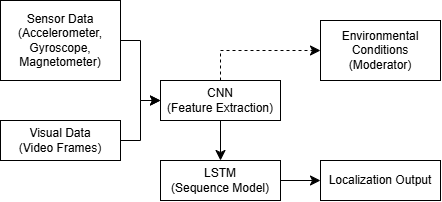
\includegraphics[width=0.7\textwidth]{figures/framework.png} 
	\caption[Conceptual Framework for the \gls{ar} Navigation System]{The Conceptual Framework for the \gls{ar} Navigation System.}
	\label{fig:thirdFig}
\end{figure}

\subsection{Data Collection}

Data collection is the foundational stage of this research, as the performance of the spatiotemporal localization model is highly dependent on the quality and consistency of the input data. The dataset that will be used in this study comprises synchronized visual and sensor data gathered from various walking paths within the \gls{cspc} campus.

Visual data will be collected using a smartphone camera held steadily to simulate a natural walking motion. To manage storage and computational demands, a hyperlapse recording strategy was employed. Instead of recording at a typical frame rate (e.g., 30 frames per second), the system captured one frame for every twenty-four frames, effectively reducing redundancy while retaining temporal relevance. This strategy ensures that only meaningful changes in the environment are retained, while still preserving enough visual continuity for temporal modeling.

In parallel with the visual data, sensor readings were logged using the smartphone’s internal sensors. This included accelerometer, gyroscope, magnetometer, and, where available, GPS data. These were sampled at a consistent rate (e.g., 50 Hz) and timestamped precisely to enable accurate alignment with video frames during preprocessing. The rotation vector sensor, in particular, was used to infer device orientation, which provides additional spatial context even when visual cues are limited.

All data will be stored locally on the device and subsequently transferred to a desktop environment for preprocessing and model training. The raw data was also annotated with location labels derived from predetermined waypoints marked on the walking path. These annotations serve as the ground truth for model training and evaluation.

By integrating both visual and sensor modalities, the collected dataset captures the spatiotemporal characteristics of user movement within the target environment, thereby enabling the model to learn patterns that correlate visual and motion data to specific locations.

\subsection{Data Pre-processing}

The collected images will undergo a series of pre\-processing steps to ensure they are suitable for training the spatiotemporal localization model. First, the images will be rescaled to a uniform resolution to maintain consistency in input dimensions across the dataset. In addition, denoising techniques will be used to reduce visual noise and enhance important features of images. Images will be augmented using techniques such as random rotation and brightness adjustments. Moreover, these images will be synchronized together with sensor data. These pre\-processing steps are essential to improve model accuracy and ensure robust performance in varying environmental conditions.

\subsection{Model Training}

The ResNet-50 model will be trained using the preprocessed image dataset to develop strong feature extraction capabilities, capturing important spatial information such as shapes, textures, and landmark details. Once trained, the high-level features extracted by ResNet-50 will be passed to the \gls{lstm} networks, which will be responsible for learning the temporal dependencies and sequential patterns across image frames. This combined \gls{cnn}-\gls{lstm} architecture will enable the system to understand both the visual context and the movement dynamics necessary for accurate spatiotemporal localization within the \gls{ar} navigation system.

\subsection{Input Sampling}

The camera will be configured to capture frames from the live stream while simultaneously listening to sensor inputs. These data will serve as input for the model trained in the previous stage. The frame sampling rate can be defined arbitrarily, such as capturing one frame for every 24 frames, depending on the system's requirements and performance considerations.

\subsection{Input Pre-processing}

Similarly with data pre-processing, input image will be rescaled. The synchronization between images and sensor data will not be computed using linear interpolation, instead it will be taken at the same time the image was captured. 

\subsection{Model Inference}

After pre-processing, the data will be passed through the trained model for inference. During this phase, ResNet-50 will extract spatial features from the image frames, while \gls{lstm} networks will process the temporal sequence and integrate contextual data from the sensors. The combined outputs of both models will be used to predict the location or spatiotemporal state of the user, providing accurate real-time navigation information.

\subsection{Performance Evaluation}

The system will be evaluated using metrics relevant to localization tasks, including accuracy, temporal consistency, latency, and robustness. Accuracy will measure how close the predicted position is to the actual one. Temporal consistency will assess how smooth and stable the predictions will be over time. The latency will evaluate how fast the model will process data in real time. Robustness will determine how well the system performs under varying lighting or motion conditions.

\subsection{Location Mapping}

The inference outputs will be mapped onto a predefined layout or map of the environment. This mapping will facilitate the visualization and application of the model predictions for navigation or tracking, ensuring that the user’s location is accurately represented in the system’s interface.

%=======================================================%
%%%%% Do not delete this part %%%%%%
\clearpage

\printbibliography[heading=subbibintoc, title={\centering Notes}]
\end{refsection}